
%(BEGIN_QUESTION)
% Copyright 2012, Tony R. Kuphaldt, released under the Creative Commons Attribution License (v 1.0)
% This means you may do almost anything with this work of mine, so long as you give me proper credit

Determine the LRV and URV settings for the water seal drum lever transmitter (LT-21), assuming the LRV point is at the lower nozzle and the URV point is at the upper nozzle (the two nozzles being 3 feet 8 inches apart from each other), and that the remote seal fill fluid has a specific gravity of 0.934:

$$\includegraphics[width=15.5cm]{i0002rx01.eps}$$

\underbar{file i02820}
%(END_QUESTION)





%(BEGIN_ANSWER)

The elevation for this transmitter (i.e. the total differential pressure applied by the height of fill fluid on both sides) is equal to the total height difference between the remote seal diaphragms multiplied by the specific gravity of the fill fluid:

$$P_{elevation} = (44 \hbox{ in})(0.934) = 41.1 \hbox{ "WC}$$

In the LRV condition, this is the only pressure seen by the transmitter.  Therefore, 41.1 "WC is the appropriate LRV setting for this transmitter.  If we assume that the ``H'' port of this DP transmitter connects to the lower nozzle, the LRV will be -44.1 "WC.  If we assume the ``H'' port connects to the upper nozzle, the LRV will be +41.4 "WC.

\vskip 10pt

In the URV condition, we have the exact same amount of elevation (the fill fluid inside the capillary tubes) but on the lower nozzle we have the hydrostatic pressure of 44 vertical inches of water (i.e. the water inside the seal drum).  Thus, in the URV condition the transmitter sees a differential pressure of:

$$P_{differential} = 44 \hbox{" WC} - 41.1 \hbox{ "WC} = 2.9 \hbox{ "WC}$$

If we assume the ``H'' port of this DP transmitter connects to the lower nozzle, the URV will be +2.9 "WC.  If we assume the ``H'' port of this DP transmitter connects to the upper nozzle, the URV will be -2.9 "WC.

$$\includegraphics[width=15.5cm]{i02820x01.eps}$$

%(END_ANSWER)





%(BEGIN_NOTES)

\vskip 20pt \vbox{\hrule \hbox{\strut \vrule{} {\bf Virtual Troubleshooting} \vrule} \hrule}

This question is a good candidate for a ``Virtual Troubleshooting'' exercise.  Presenting the diagram to students, you first imagine in your own mind a particular fault in the system.  Then, you present one or more symptoms of that fault (something noticeable by an operator or other user of the system).  Students then propose various diagnostic tests to perform on this system to identify the nature and location of the fault, as though they were technicians trying to troubleshoot the problem.  Your job is to tell them what the result(s) would be for each of the proposed diagnostic tests, documenting those results where all the students can see.

During and after the exercise, it is good to ask students follow-up questions such as:

\begin{itemize}
\item{} What does the result of the last diagnostic test tell you about the fault?
\item{} Suppose the results of the last diagnostic test were different.  What then would that result tell you about the fault?
\item{} Is the last diagnostic test the best one we could do?
\item{} What would be the ideal order of tests, to diagnose the problem in as few steps as possible?
\end{itemize}

%INDEX% Measurement, level: hydrostatic pressure
%INDEX% Process: steam-heated reactor vessel (generic)

%(END_NOTES)


